\section{Cara Mengimplementasikan Jinja pada Flask}
Flask memanfaatkan Jinja2 sebagai mesin template. Di sinilah orang dapat mengambil keuntungan dari mesin template Jinja2, di mana Flask didasarkan. Istilah 'sistem templating web merujuk pada merancang skrip HTML tempat data variabel dapat dimasukkan secara dinamis. Template web berisi sintaks HTML yang diselingi placeholder untuk variabel dan ekspresi (dalam hal ini ekspresi Python) yang merupakan nilai yang diganti saat template diberikan.

Jinja2 adalah mesin templat yang ditulis dengan Python murni, Ini kecil tapi cepat, selain menjadi mesin template mandiri yangsimple dan mudah digunakan. Flask adalah kerangka kerja web mikro berbasis Python yang memungkinkan Anda menulis aplikasi web dengan cepat dan efisien. Dasar-dasar Jinja2 templating dari perspektif Flask menata templat dalam aplikasi berbasis Flask dalam desain modular dan dapat diperluas.
\begin{enumerate}
\item Pastinya anda sudah memiliki pemahaman dasar tentang Flask dan pengaturan lingkungan praktik terbaik menggunakan virtualenv yang harus diikuti saat mengembangkan aplikasi Python. Sebelumnya anda sudah mempelajari cara instalasi micro-framework flask dan membuat aplikasi sederhana. Secara umum framework menyediakan template engine bawaan, dalam hal ini flask dengan jinja2.   
\item Untuk memahami konsep dan cara kerja template contoh dibawah akan menunjukkan sebuah aplikasi sederhana dengan tag html dan tipe data python dictionary pada sebuah route flask yang sudah dibuat sebelumnya.

Dalam Flask, anda dapat menulis aplikasi web yang lengkap tanpa perlu mesin templating pihak ketiga. Mari  Anda lihat aplikasi app.py seperti pada listing \ref{lst:app}:
\lstinputlisting[caption=File app.py,label={lst:app}]{src/13/app.py}

\item Simpan kode diatas dengan nama app,py kemudian jalankan program python diatas di cmd seperti pada gambar \ref{fig:uap}.
\begin{figure}[!htbp]
	\centerline{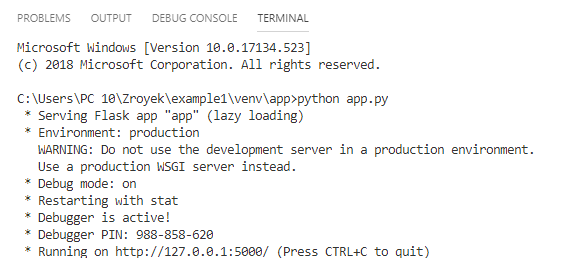
\includegraphics[width=0.85\textwidth]{figures/13/uap.PNG}}
	\caption{Pengujian app.py}
	\label{fig:uap}
\end{figure}

\item Setelah itu akan muncul pemberitahuan bahwa Flask telah berjalan di localhost.
\item Jalankan program di http://127.0.0.1:5000/ maka akan muncul halaman web seperti pada gambar \ref{fig:hufa}.
\begin{figure}[!htbp]
	\centerline{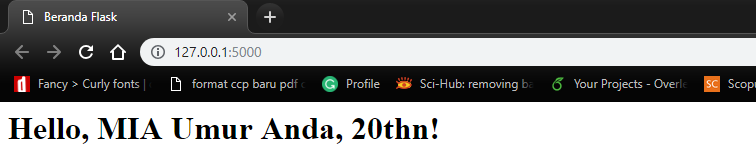
\includegraphics[width=0.85\textwidth]{figures/13/hufa.PNG}}
	\caption{Hasil Pengujian File app.py}
	\label{fig:hufa}
\end{figure}

\item “orang = \{'nama': 'MIA', 'umur':'20thn'\}” ini adalah dictionary yang dibuat dan akan digunakan dan di masukan kedalam aplikasi flask yang akan di buat.
\item Nama MIA ditampilkan di browser karna ‘mia’ ada di dalam dictionary yang sudah dibuat pada kode diatas begitupul dengan umur yang di tampilkan di browser seperti pada listing \ref{lst:appe}:
\lstinputlisting[caption=File app.py edit,label={lst:appe}]{src/13/appe.py}

\item Kemudian ini merupakan body atau isi yang sudah dibuat yang kemudian di tampilkan di web browser. [‘nama’] akan dipanggil sesuai dengan dictionary yang sudah dibuat begitu juga dengan umur, jika nama dan umur  Anda ubah maka apa yang di tampilkan di browser juga terubah.
Contoh :
\item Misalnya dictionary “orang = \{'nama': 'MIA', 'umur':'20thn'\}” diubah menjadi 
“orang = \{'nama': 'Novi BB', 'umur':'19thn'\}”
 \item kemudian jalankan kembali program yang sudah diubah.
\item jalankan program python diatas di cmd seperti pada gambar \ref{fig:pae}.
\begin{figure}[!htbp]
	\centerline{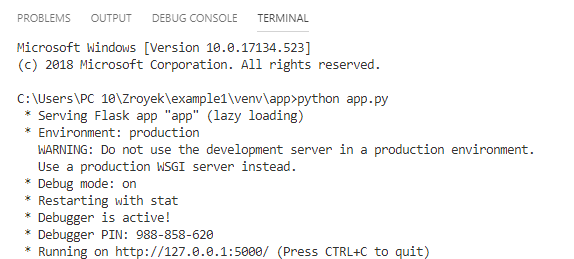
\includegraphics[width=0.85\textwidth]{figures/13/pae.PNG}}
	\caption{Pengujian File app.py edit}
	\label{fig:pae}
\end{figure}

\item Setelah itu akan muncul pemberitahuan bahwa Flask telah berjalan di localhost.
\item Jalankan program di http://127.0.0.1:5000/ maka akan muncul halaman web seperti pada gambar \ref{fig:hpae}.
\begin{figure}[!htbp]
	\centerline{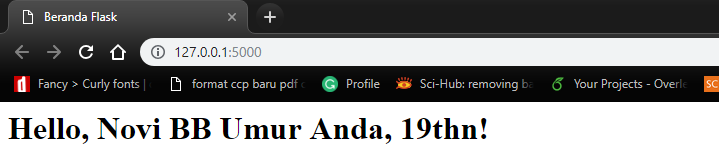
\includegraphics[width=0.85\textwidth]{figures/13/hpae.PNG}}
	\caption{Hasil Pengujian File app.py edit}
	\label{fig:hpae}
\end{figure}

\item Jika nama di ganti didalam dictionary yang sudah dibuat maka tampilan web yang akan muncul sesuai dengan nama yang ada di dalam dictionary.
\end{enumerate}

Contoh diatas kurang efektif untuk membuat suatu aplikasi yang nantinya akan memiliki banyak function dan kode lainnya  Aplikasi juga akan memiliki lebih banyak view function dengan semakin banyaknya URL yang akan di buat, jadi bayangkan jika suatu hari nanti  Anda akan mengubah salah satu layout, maka  Anda harus memperbarui HTML di view function lainnya. Maka dari itu flask menyediakan jinja2 sebagai template untuk mempermudah dalam memodifikasi aplikasi yang akan teman teman bangun. 

Jinja2 sudah include pada saat  Anda install flask, sehingga  Anda tidak perlu lagi melakukan konfigurasi /modifikasi apapun di terminal. Memang flask mengizinkan  Anda untuk menggunakan template engine lainnya akan tetapi yang paling popular digunakan pada flask adalah jinja2.

Templates membantu mencapai pemisahan antara presentation dan business logic. Di Flask, template ditulis sebagai file yang berbeda, disimpan di folder templates yang ada di dalam application package. Jadi setelah memastikan  Anda berada di direktori microblog, buat direktori untuk menyimpan templates:
\begin{enumerate}
\item Buat folder baru bernama templates didalam package tempat anda menyimpan program. 
\item Kemudian buat file baru bernama index.html dalam folder template sehingga struktur projek yang akan di buat seperti pada gambar \ref{fig:sp}.
\begin{figure}[!htbp]
	\centerline{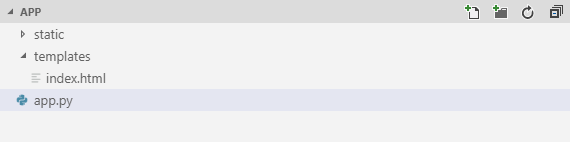
\includegraphics[width=0.85\textwidth]{figures/13/sp.PNG}}
	\caption{Struktur Projek}
	\label{fig:sp}
\end{figure}

\item Sekarang mari  Anda modifikasi file yang  Anda buat sebelumnya. 
\item File index.html akan di modifikasi seperti pada listing \ref{lst:indx}:
\lstinputlisting[caption=File index.html,label={lst:indx}]{src/13/index.html}
 
\item Simpan scrip html dengan nama index.html didalam folder template.
\item Kode html diatas sangat standar satu-satunya kode yang perlu anda ketahui mengenai jinja adalah kode yang diapit kurung keriting \{\{ … \}\} didalam tanda tersebut  Anda letakkan variabel python. 
\item Kemudian edit juga file app.py yang sudah dibuat sebelumnya seperti pada listing \ref{lst:appe2}:
\lstinputlisting[caption=File app.py edit 2,label={lst:appe2}]{src/13/appe2.py}
 
\item Operasi yang mengubah sebuah template menjadi halaman HTML utuh disebut dengan rendering. 
\item Untuk me-render template  Anda harus mengimpor sebauh fungsi Flask bernama render\_template(). 
\item Fungsi ini meminta nama file template dan daftar variabel python yang diapit kurung keriting \{\{ … \}\} yang ada di  file index.html dalam folder templates tersebut.
\item Funsi render\_template() juga memanggil template engine bernama Jinja2 yang sudah ada bersama dengan framework Flask. 
\item Jinja2 mengganti blok \{\{ ... \}\} menjadi nilai yang diinginkan menggunakan argumen yang  Anda tulis di pemanggilan render\_template().
\item Selanjutnya  Anda akan mencoba menjalankan program yang sudah di modifikasi
\item Simpan kode file app.py kemudian jalankan program python diatas di cmd seperti pada gambar \ref{fig:ufa}.
\begin{figure}[!htbp]
	\centerline{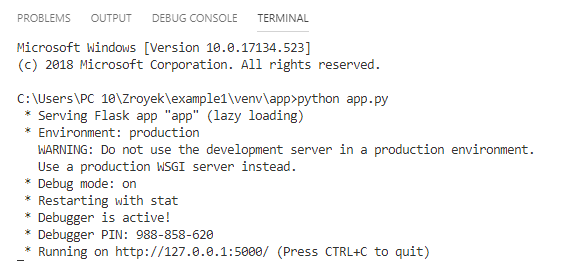
\includegraphics[width=0.85\textwidth]{figures/13/ufa.PNG}}
	\caption{Pengujian file app.py edit 2}
	\label{fig:ufa}
\end{figure}

\item Setelah itu akan muncul pemberitahuan bahwa Flask telah berjalan di localhost.
\item Jalankan program di http://127.0.0.1:5000/ maka akan muncul halaman web seperti pada gambar \ref{fig:hufa2}.
\begin{figure}[!htbp]
	\centerline{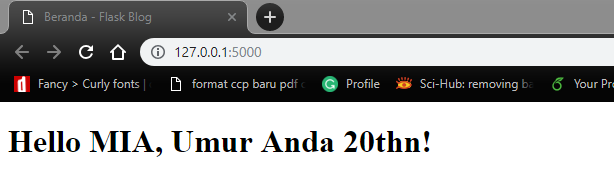
\includegraphics[width=0.85\textwidth]{figures/13/hufa2.PNG}}
	\caption{Hasil Pengujian file app.py edit 2}
	\label{fig:hufa2}
\end{figure}

Flask akan merender file index.html didalam folder templates dengan memanggil modul render\_template secara otomatis jinja2 akan memanggil file index.html dalam folder templates dan menampilkannya di browser dengan URL http://127.0.0.1:5000/  yang telah disediakan oleh flask. Hampir sama dengan contoh sebelumnya yang mana kode html yang disatukan dengan kode flask dan menggunakan dictionary yang dibuat untuk mendefinisikan sebuah variable nama dan umur yang akan di tampilkan di web browser.

Bedanya kode html dipisahkan kedalam folder templates yang dibuat secara dinamis dan di dalam kode flask dipanggil menggunakan modul render\_template(). Kemudian flask akan memanfaatkan jinja2 untuk memanggil file index.html yang ada pada folder templates. Di dalam kode index.html digunakan sebuah variable yang di masukan didalam kurung capit \{\{….\}\} agar jinja2 dapat mengetahui apa yang akan di panggil dan di tampilkan ke browser. Dan di dalam kode flask app.py masih harus menggunakan dictionary agar dapar mendefinisikan sebuah variael yang sudah dibuat. Kuncinya ada di dalam dictionary yang dibuat pada file app.py
\verb|“orang = \{'nama': 'MIA', 'umur':'20thn'\}”|

\item Dictionary di letakan di dalam fungsi yang dibuat 
\item Dan didalam file index.html  seperti pada listing \ref{lst:idx}:
\lstinputlisting[caption=File index.html,label={lst:idx}]{src/13/indx.html}

\item Ini merupakan isi dari apa yang akan di tampilkan di browser, pada browser akan menampilkan kalimat “Hello MIA, Umur Anda 20 thn”
\item Dan menggunakan heading 1 agar kalimat yang ditampilkan di browser jelas.
\item \{\{orang.nama\}\} variable ini menampilkan nama orang yang ada di dictionary ‘orang’ yang sudah dibuat.
\item Begitupula dengan \{\{orang.umur\}\} akan  menampilkan umur yang sudah di seting di dalam dictionary yang sudah dibuat.
\item Kemudian didalam file app.py tentunya menggunakan modull render\_template().
\item Dan mengembalikan fungsi yang sudah dibuat dengan menambahkan kode 
\item ‘return render\_template('index.html', title='Beranda', orang=orang)’
\item Kode tersebut akan menampilkan file index.html dengan cara merender dari folder template dengan menggunakan modul render\_template().
 \item Kemudian mengatur tilte dengan kalimat ‘beranda’, dan menampilkan kalimat yang sudah di seting di file index.html
 \item Dengan memanggil dictionary yang sudah si buat di file app.py
\item Kemudian flask akan memanfaatkan jinja2 yang bekerja sebagai render template file index.html.
\item File index.html bisa  Anda edit agar tampilan yang ada dibroeser menjadi lebih menarik untuk dilihat
\item Anda bisa menambahkan css untuk mengedit tampilan pada web browser tapi dengan output yang sama 
\item Bisa juga dengan menggunakan bootstrap agar tampilan web lebih menarik untuk di pandang.
\item Sekarang teman teman bisa menambahkan file css yang nanti akan  Anda buat untuk mempercantik tulisan yang akan di tampilkan di web browser.
\item Edit file index.html didalam folder templates dan kemudian tambahkan contoh code css untuk mengubah tampilan yang akan di tampilkan di browser seperti pada listing \ref{lst:ine1}:
\lstinputlisting[caption=File index.html edit 1,label={lst:ine1}]{src/13/ine1.html}

\item Simpan code index.html diatas, kemudian untuk file app.py tidak ada yang di modifikasi.
\item Kemudian jalankan flask seperti biasa di cmd dengan menjalankan file app.py dengan perintah python app.py seperti pada gambar \ref{fig:ufa2}.
\begin{figure}[!htbp]
	\centerline{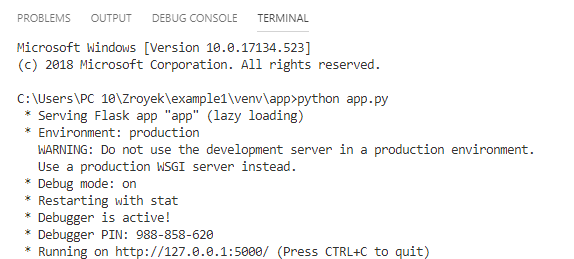
\includegraphics[width=0.85\textwidth]{figures/13/ufa2.PNG}}
	\caption{Pengujian file app.py edit 2}
	\label{fig:ufa2}
\end{figure}

\item Setelah itu akan muncul pemberitahuan bahwa Flask telah berjalan di localhost.
\item Jalankan program di http://127.0.0.1:5000/ maka akan muncul halaman web seperti pada gambar \ref{fig:hufae2}.
\begin{figure}[!htbp]
	\centerline{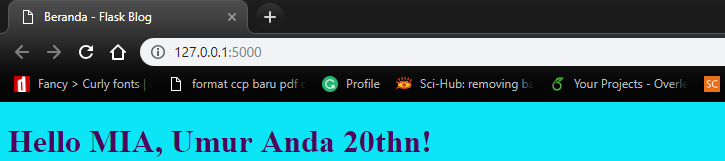
\includegraphics[width=0.85\textwidth]{figures/13/hufae2.PNG}}
	\caption{Hasil Pengujian file app.py edit 2}
	\label{fig:hufae2}
\end{figure}

\item Tampilan pada file index.html didalam folder template dapat  Anda modifikasi sesuai selera  Anda, dan pada saat program dijalankan tentunya tidak akan jadi masalah dengan program yang sudah  Anda buat selama ketika memodifikasi file index.html tidak ada salah kata atau kuran tanda dalam kode yang  Anda modifikasi.
\item Flask akan menggunakan jinja2 dalam hal merender template dan memanggil file index.html.
\item Selama variable dalam file index.html tidak ada yang berubah dan tetap mendefinisikan variable yang ada pada dictionary flask.
\item Kalaupun ada yang bermasalah (Error) flask akan memberi tahu dimana letak kesalahan yang terjadi.
Contoh seperti pada listing \ref{lst:ine2}:
\lstinputlisting[caption=File index.html edit 2,label={lst:ine2}]{src/13/ine2.html}

\item Anda akan sedikit merubah kode di bagian yang dijadikan variable 
\item \verb|<h1>Hello \{\{ orang.nama\}, Umur Anda \{\{ orang.,umur \}\}!</h1>|
\item Simpan code index.html diatas Kemudian jalankan flask seperti biasa di cmd dengan menjalankan file app.py dengan perintah python app.py seperti pada gambar \ref{fig:ufae}.
\begin{figure}[!htbp]
	\centerline{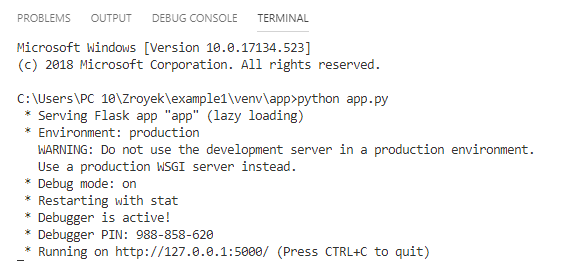
\includegraphics[width=0.85\textwidth]{figures/13/ufae.PNG}}
	\caption{Pengujian file app.py edit 2}
	\label{fig:ufae}
\end{figure}

\item Setelah itu akan muncul pemberitahuan bahwa Flask telah berjalan di localhost.
\item Jalankan program di http://127.0.0.1:5000/ maka akan muncul halaman web seperti pada gambar \ref{fig:hufae}.
\begin{figure}[!htbp]
	\centerline{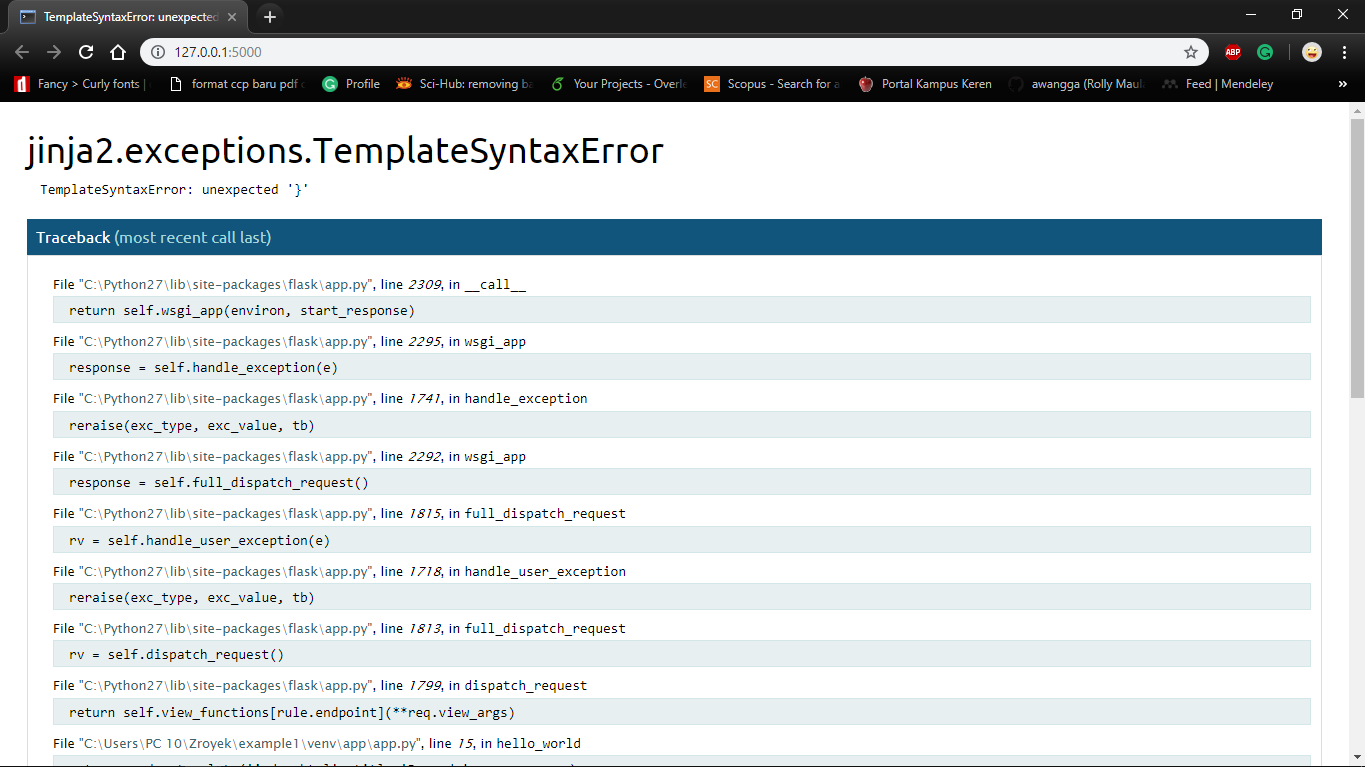
\includegraphics[width=0.85\textwidth]{figures/13/hufae.PNG}}
	\caption{Hasil Pengujian file app.py edit 2}
	\label{fig:hufae}
\end{figure}

\item Maka terjadilah eror seperti gambar diatas.
\item Jinja2 pada flask memberitahu bahwa ada syntak eror dalam file template yang di render
\item Syntax yang eror adalah sebagai berikut 
\verb|TemplateSyntaxError: unexpected '\}'|
\item Jinja2 flask memberitahu bahwa di dalam file index.html terjadi hal tak terduga atau bisa dibilang salah satu kode yang mendefinisikan variable pada flask tidak ada.
\item Sehingga jinja2 tidak bisa merender file index.html di dalam folder template dengan benar.
\item Anda akan memperbaiki kesalahan yang  Anda buat, ini hanya sekedar contoh saja  seperti pada listing \ref{lst:ine3}:
\lstinputlisting[caption=File index.html edit 3,label={lst:ine3}]{src/13/ine3.html}

\item Menambahkan kurung kurung keriting  untuk menjadikannya sebuah variable kembali.
\item Simpan code index.html diatas Kemudian jalankan flask seperti biasa di cmd dengan menjalankan file app.py dengan perintah python app.py seperti pada gambar \ref{fig:ufae2}.
\begin{figure}[!htbp]
	\centerline{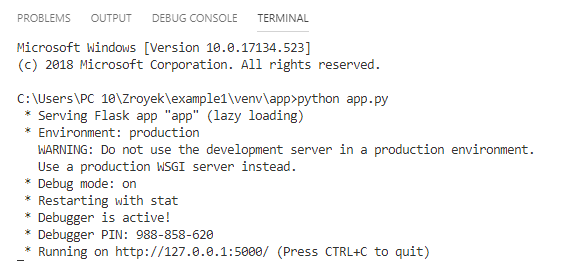
\includegraphics[width=0.85\textwidth]{figures/13/ufae2.PNG}}
	\caption{Pengujian file app.py edit 2}
	\label{fig:ufae2}
\end{figure}

\item Setelah itu akan muncul pemberitahuan bahwa Flask telah berjalan di localhost.
\item Jalankan program di http://127.0.0.1:5000/ maka akan muncul halaman web seperti pada gambar \ref{fig:hfae}.
\begin{figure}[!htbp]
	\centerline{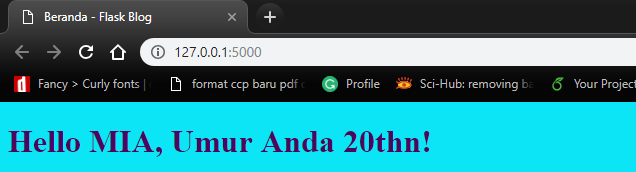
\includegraphics[width=0.85\textwidth]{figures/13/hfae.PNG}}
	\caption{Hasil Pengujian file app.py edit 2}
	\label{fig:hfae}
\end{figure}

\item Selain mengubah tampilan dengan memasukan kode css kedalam file index.html seperti yang dilakukan sebelumnya, file index.html bisa anda tambahkan dengan boostrap agar tampilan pada web browser lebih menarik untuk dipandang.
\item Teman teman bisa mengunjungi situs yang menyediakan boostrap untuk tampilan web sederhana.
\item Sebagai contoh disini akan menambahkan boostrap sederhana dari situs yang menyediakan bostrap tersebut 
\item Anda modifikasi file index.html seperti pada listing \ref{lst:ine4}:
\lstinputlisting[caption=File index.html edit 4,label={lst:ine4}]{src/13/inn.html}

\item Simpan file index.html yang telah dimodifikasi dan ditambahkan dengan boostrap sederhana.
\item Kemudian jalankan flask seperti biasa di cmd dengan menjalankan file app.py dengan perintah python app.py seperti pada gambar \ref{fig:ufaa}.
\begin{figure}[!htbp]
	\centerline{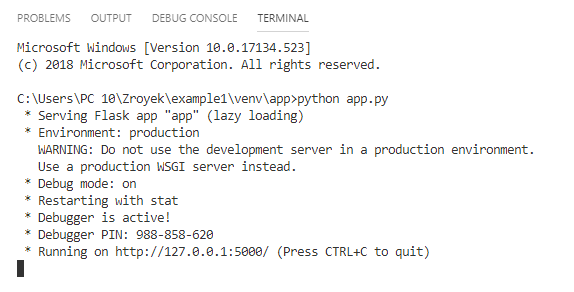
\includegraphics[width=0.85\textwidth]{figures/13/ufaa.PNG}}
	\caption{Pengujian file app.py edit 2}
	\label{fig:ufaa}
\end{figure}

\item Setelah itu akan muncul pemberitahuan bahwa Flask telah berjalan di localhost.
\item Jalankan program di http://127.0.0.1:5000/ maka akan muncul halaman web seperti pada gambar \ref{fig:hufaa}.
\begin{figure}[!htbp]
	\centerline{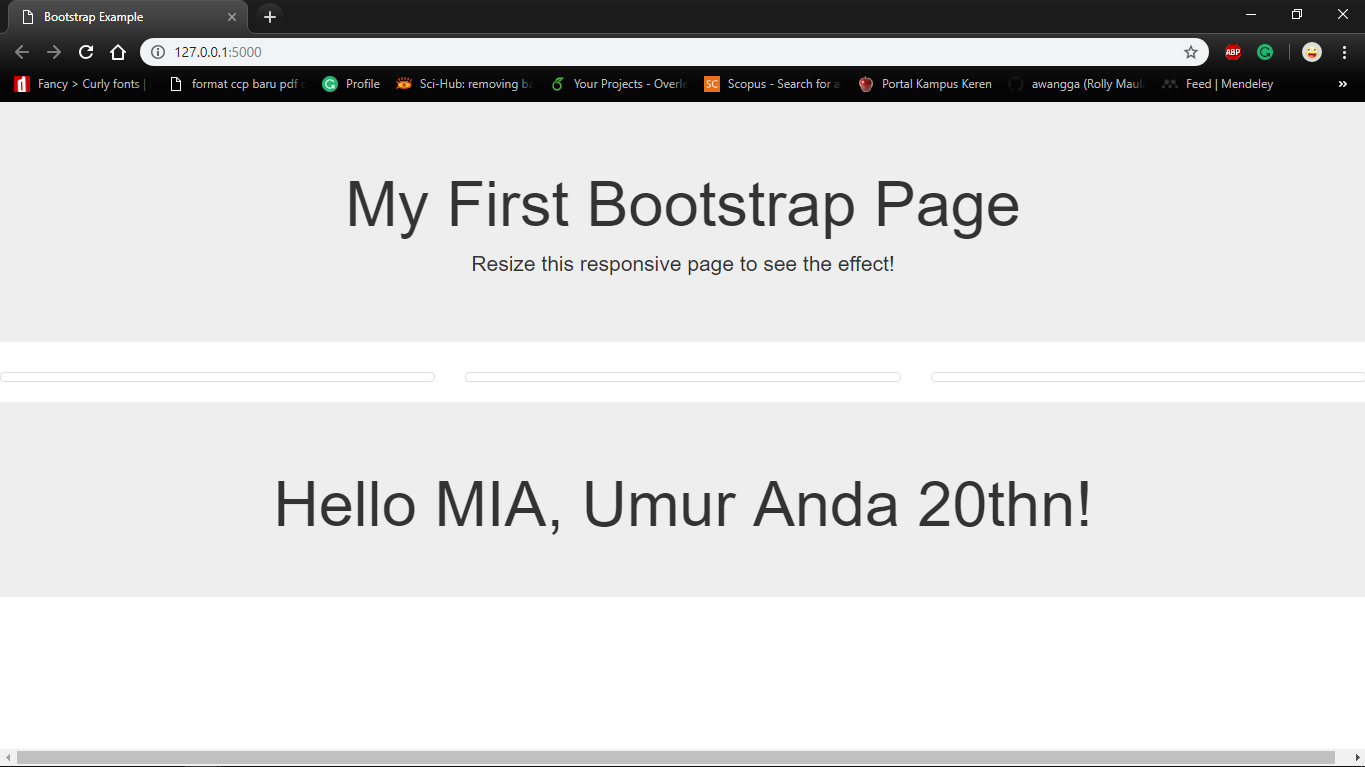
\includegraphics[width=0.85\textwidth]{figures/13/hufaa.PNG}}
	\caption{Hasil Pengujian file app.py edit 2}
	\label{fig:hufaa}
\end{figure}

\item Ini adalah tampilan dari file yang sudah dimodifikasi sebelumnya, jinja2 flask tetap merender file html yang di modifikasi menampilkan kalimat sapaan kepada user MIA.
\item Selama penggunaan variable pada file html dilakukan dengan benar maka jinja2 flask akan melakukan tugasnya dengan benar:
\begin{verbatim}
<div class="jumbotron text-center">
<h1>Hello \{\{ orang.nama\}\}, Umur Anda \{\{ orang.umur \}\}!</h1>
</div>
\end{verbatim}

\item Bukan hanya nama MIA saja yang bisa di tampilkan di web browser  Anda juga mengubah nama  Anda dengan sesuka hati
\item Caranya hanya dengan mengubah nama di file app.py di bagian dictionary yang dibuat untuk mendefinisikan nama yang akan di tampilkan.

Contoh seperti pada listing \ref{lst:appe3}:
\lstinputlisting[caption=File app.py edit 3,label={lst:appe3}]{src/13/appe3.html}:

\item Anda akan mengubah nama MIA menjadi nama Orang lain 
\verb|orang = \{'nama': 'Orang lain', 'umur':'21thn'\}|
\item Simpan kode app.py yang sudah di modifikasi kemudian jalankan program python diatas di cmd seperti pada gambar \ref{fig:ufa3}.
\begin{figure}[!htbp]
	\centerline{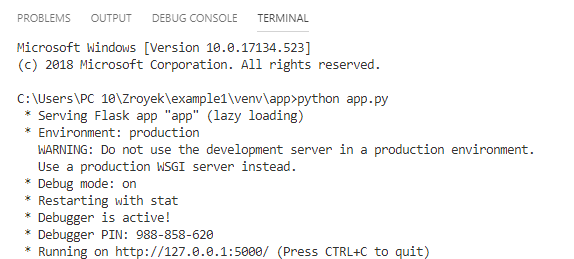
\includegraphics[width=0.85\textwidth]{figures/13/ufa3.PNG}}
	\caption{Pengujian file app.py edit 3}
	\label{fig:ufa3}
\end{figure}

\item Setelah itu akan muncul pemberitahuan bahwa Flask telah berjalan di localhost.
\item Jalankan program di http://127.0.0.1:5000/ maka akan muncul halaman web seperti pada gambar \ref{fig:hufa3}.
\begin{figure}[!htbp]
	\centerline{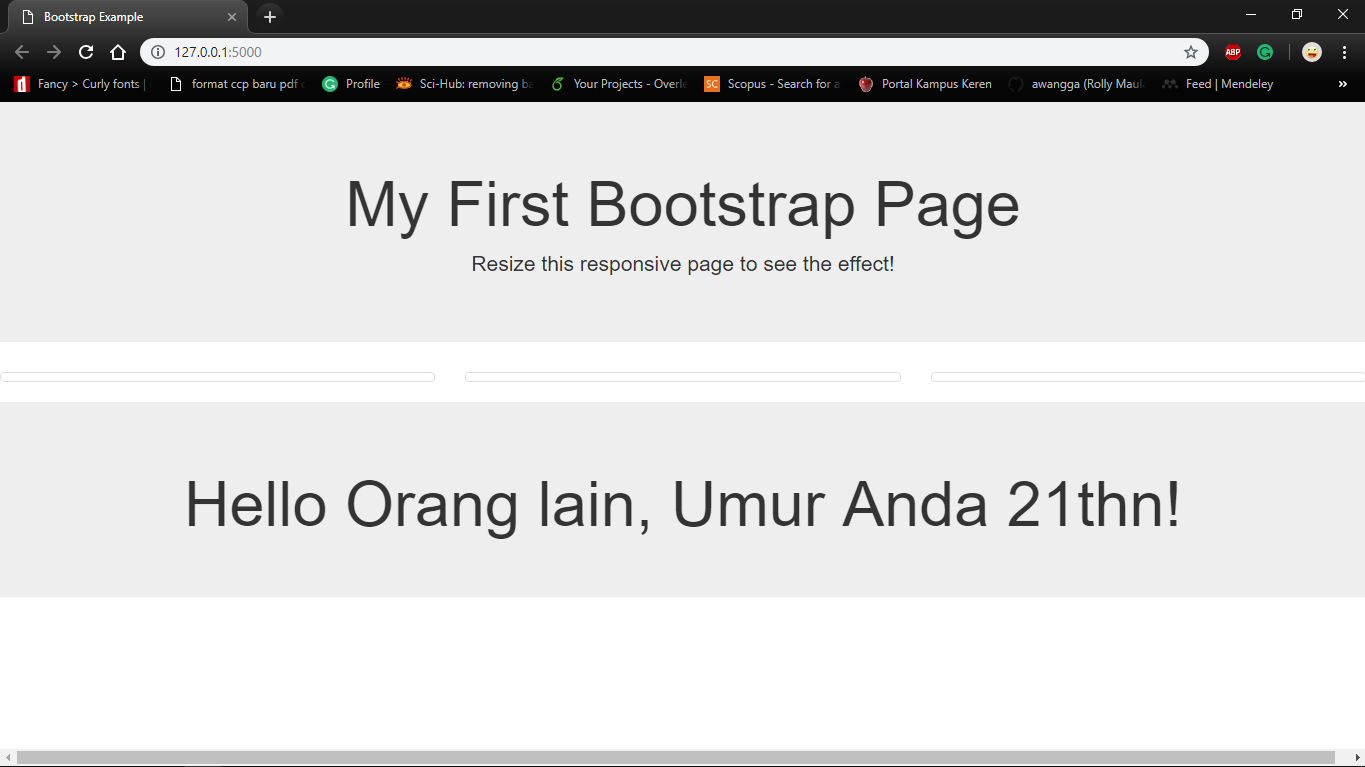
\includegraphics[width=0.85\textwidth]{figures/13/hufa3.PNG}}
	\caption{Hasil Pengujian file app.py edit 3}
	\label{fig:hufa3}
\end{figure}

\item Itulah tadi cara mengimplementasikan Jinja2 di flask.
\end{enumerate}

\section{Penanganan Error}
Flask adalah sebuah Micro Web Framework yang ditulis menggunakan Bahasa Pemrograman Python. Flask sendiri berlisensi BSD.
Untuk mengetahui atau anda ingin mempelajari Flask bisa mengunjungi halaman web doc dari flask http://flask.pocoo.org . Disana telah disediakan semua tentang Flask. Mulai dari instalasi Flask sampai menggunakan Modul yang tersedia pada Flask.

Kode dibawah merupakan kode program yang sudah dibuat. Program yang sudah dibuat merupakan program yang menggunakan bahas pemograman python dan menggunakan framework flask. Sebagai contoh eror pada program yang sudah dibuat seperti pada listing \ref{lst:flcs}:
\lstinputlisting[caption=File flasklivechart.py,label={lst:flcs}]{src/13/flcs.py}

\begin{enumerate}
\item Simpan skrip kode diatas kemudian namakan file tersebut menjadi flasklivechart.py, jalankan file tersebut menggunakan cmd dengan menuliskan perintah python flasklivechart.py seperti pada gambar \ref{fig:uflc}.
\begin{figure}[!htbp]
	\centerline{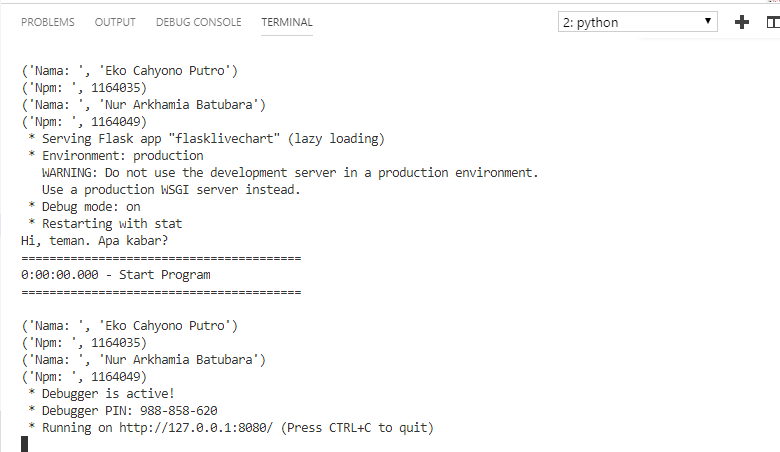
\includegraphics[width=0.85\textwidth]{figures/13/uflc.PNG}}
	\caption{Pengujian file flasklivechart.py}
	\label{fig:uflc}
\end{figure}

\item Setelah itu akan muncul pemberitahuan bahwa Flask telah berjalan di localhost.
\item Jalankan program di http://127.0.0.1:8080 kemudian akan muncul tampilan seperti pada gambar \ref{fig:huflc}.
\begin{figure}[!htbp]
	\centerline{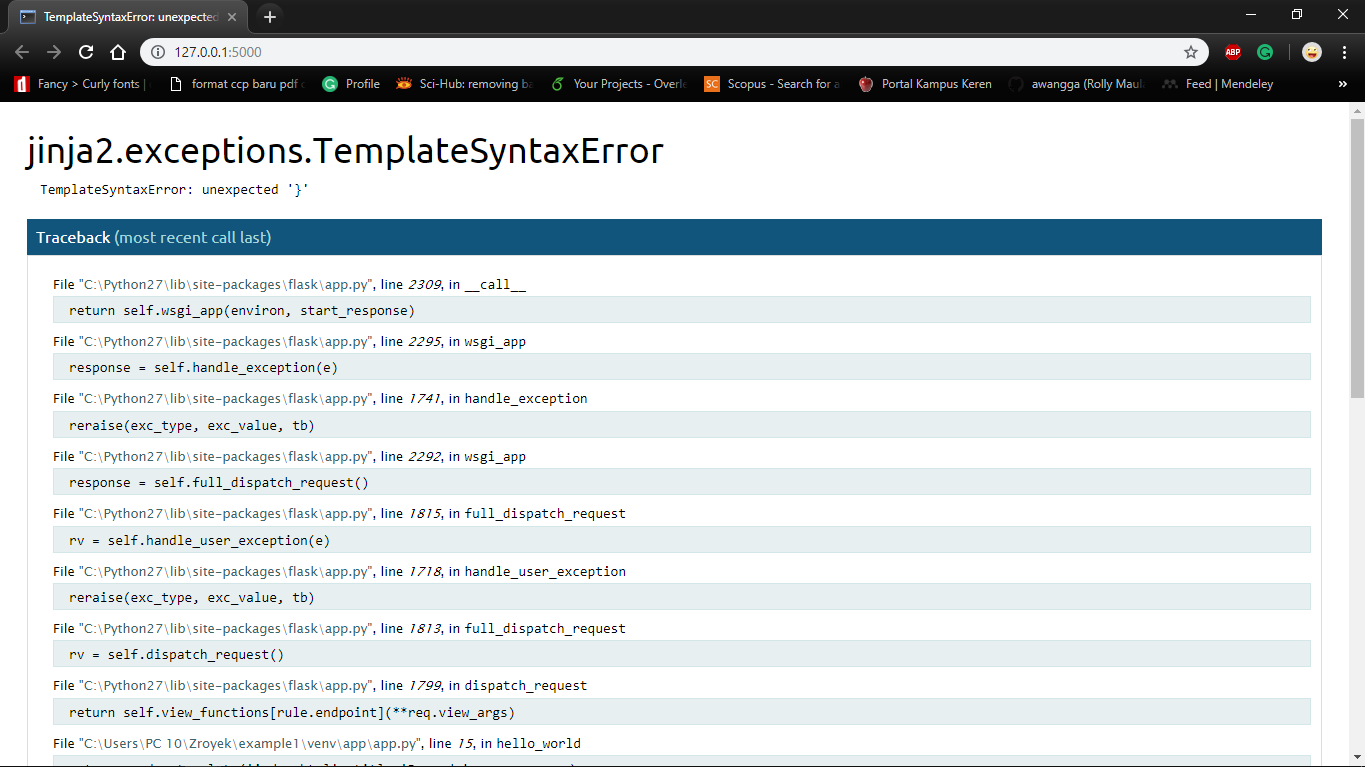
\includegraphics[width=0.85\textwidth]{figures/13/huflc.PNG}}
	\caption{Hasil Pengujian file flasklivechart.py}
	\label{fig:huflc}
\end{figure} 

\item Maka terjadilah eror seperti gambar diatas.
\item Jinja2 pada flask memberitahu bahwa ada syntak eror dalam file template yang di render. Syntax yang eror adalah sebagai berikut:
\verb|TemplateSyntaxError: unexpected '\}'|
\item Jinja2 flask memberitahu bahwa di dalam file index.html terjadi hal tak terduga atau bisa dibilang salah satu kode yang mendefinisikan variable pada flask tidak ada. Sehingga jinja2 tidak bisa merender file index.html di dalam folder template dengan benar.
\item Dan untuk file indek html adalah seperti pada listing \ref{lst:ind}:
\lstinputlisting[caption=File index.html,label={lst:ind}]{src/13/ind.py}

\item Di dalam kode index.html digunakan sebuah variable yang di masukan didalam kurung capit \{\{….\}\} agar jinja2 dapat mengetahui apa yang akan di panggil dan di tampilkan ke browser.
\item Kita akan coba memperbaiki kesalahan yang terjadi pada index.html:
\verb|<img src ="\{\{ user\_image \}\}" alt ="user\_image">|
\item Tambahkan kurung kurawa tutup pada script kode kemudian save file yang sudah dimodifikasi
\item Setelah itu jalankan kembali program tersebut seperti pada gambar \ref{fig:ujif}.
\begin{figure}[!htbp]
	\centerline{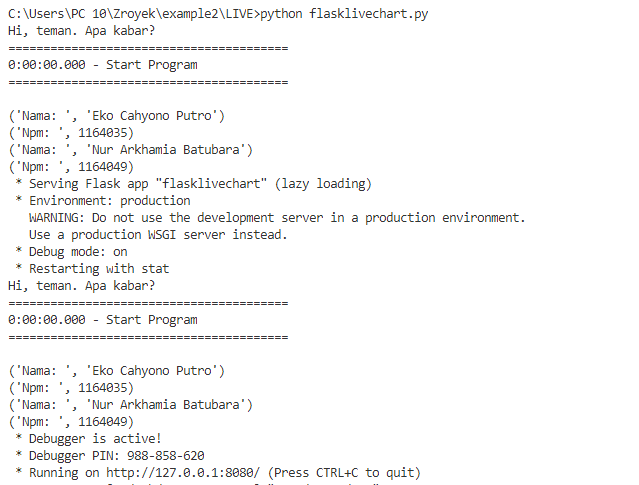
\includegraphics[width=0.85\textwidth]{figures/13/ujif.PNG}}
	\caption{Pengujian file flasklivechart.py}
	\label{fig:ujif}
\end{figure}

\item Setelah itu akan muncul pemberitahuan bahwa Flask telah berjalan di localhost.
\item Jalankan program di http://127.0.0.1:8080 kemudian akan muncul tampilan seperti pada gambar \ref{fig:huji}.
\begin{figure}[!htbp]
	\centerline{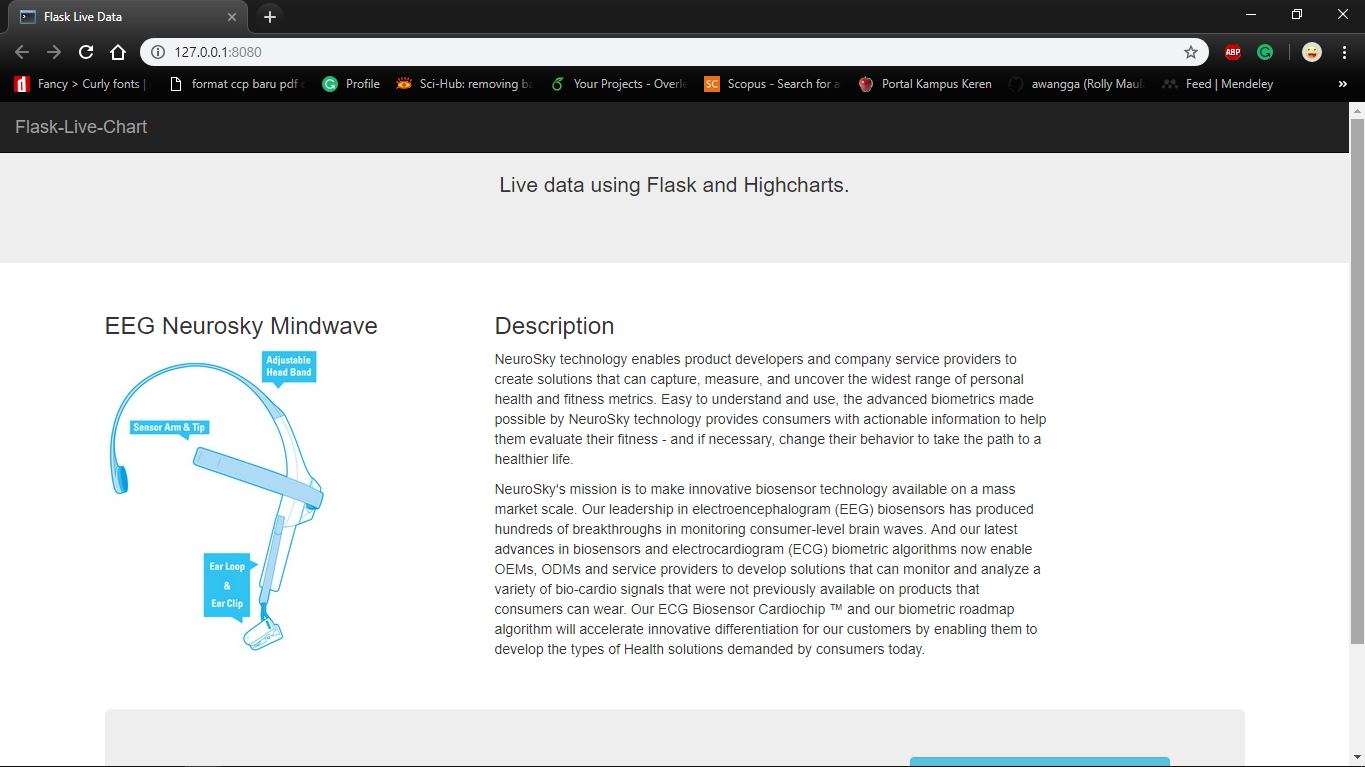
\includegraphics[width=0.85\textwidth]{figures/13/huji.PNG}}
	\caption{Hasil Pengujian file flasklivechart.py}
	\label{fig:huji}
\end{figure}

\item Akhirnya program program sudah bisa di jalankan kembali.
Kesalahan yang terjadi sebelumnya kenapa sampai bisa terjadi eror adalah pada file indek.html yang dijadikan sebagai tampilan untuk halaman web terdapat suatu kesalahan dimana variable yang di gunakan kurang lengkap. Flask akan merender file index.html didalam folder templates dengan memanggil modul render\_template secara otomatis jinja2 akan memanggil file index.html dalam folder templates dan menampilkannya di browser. Halam web yang ditampilkan seperti pada gambar diatas merupakan halam web dari program yang sudah dibuat.  Dan pada halam web terdapat sebuah button yang akan mengarah ke dalam program yang akan dijalankan.

\end{enumerate}